\documentclass[fr]{../../../../../../eplexam}

\usepackage{tikz}
\usepackage{systeme}

\hypertitle{Mécanique des Fluides}{6}{MECA}{1321}{2018}{Juin}{Majeure}
{Martin Braquet}
{Vincent Legat et Grégoire Winckelmans}

\section{Partie VL}

On considère l'écoulement d'huile (fluide visqueux newtonien) le long d'une plaque plane. Hormis une pression extérieure notée $p_0$, la surface est libre de contraintes. Une couche limite de hauteur $\delta(x)$ apparait en $x=0$ et atteint la hauteur $h(x)$ du flux d'huile en $x=L$. La région en dehors de cette couche limite est irrotationnelle. La vitesse de l'huile est constante en $x=0$ et est notée $U_0$, la hauteur de l'huile vaut $h_0$ à cet endroit. La hauteur du flux d'huile est nettement inférieur à la longueur de la plaque: $h(x)<<L$.

\begin{center}
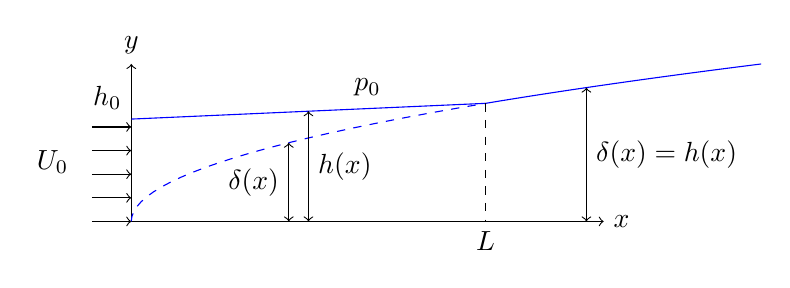
\begin{tikzpicture}
    \draw[->] (0,0) -- (6,0) node[right] {$x$};
    \draw[->] (0,0) -- (0,2) node[above] {$y$};
    \draw[domain=0:1.5,dashed,variable=\x,blue] plot ({2*\x*\x},{\x});
    \draw[domain=1.5:2,smooth,variable=\x,blue] plot ({2*\x*\x},{\x});
    \draw[blue] (0,1.3) -- (4.5,1.5);
    \draw (0,1.3) node [above left] {$h_0$};
    \draw[dashed] (4.5,1.5) -- (4.5,0) node [below] {$L$};
    \draw (3,1.7) node {$p_0$};
    \draw[<->] (2.25,0) -- node[right] {$h(x)$} (2.25,1.4) ;
    \draw[<->] (2,1) -- node[left] {$\delta(x)$} (2,0) ;
    \draw[<->] (5.78,1.7) -- node[right] {$\delta(x)=h(x)$} (5.78,0) ;
    \foreach \i in {0,0.3,...,1.5}
        \draw[->] (-0.5,\i) -- (0,\i);
        
    \draw (-1,0.75) node {$U_0$};
\end{tikzpicture}
\end{center}

Les équations régissant ce problème s'expriment donc 
\[
\systeme*{\frac{\partial u}{\partial x} + \frac{\partial v}{\partial y}=0,\rho u\frac{\partial u}{\partial x}+\rho v\frac{\partial u}{\partial y}= -\frac{\partial p}{\partial x}+\mu\frac{\partial^2 u}{\partial x^2}, \frac{\partial p}{\partial y}=\rho g}
\]

\begin{enumerate}
 \item Dessiner le profil de vitesse en $x=L/2$.
 \item Donner un ordre de grandeur pour $v(x,y)$.
 \item Trouver $p(x,y)$.
 \item Donner les conditions limites en $y=0,y=\delta$ et $y=h(x)$.
 \item Déterminer les constantes $a$ et $b$ telles que pour $x>L$,
 \[
  \frac{u(x,y)}{U(x)}=a\left(\frac{y}{\delta}\right)+b\left(\frac{y}{\delta}\right)^3
 \]
 où $U(x)=u(x,\delta(x))$.
 \item En utilisant la conservation du flux d'huile, trouver la constante $c$ telle que 
 \[
  c=\frac{U_0 h_0}{U_L h_L}
 \]
 où $U_L=U(l)$ et $h_L=h(L)$.
 \item Démontrer l'équation de Bernouilli dans le cas bidimensionnel, c'est-à-dire que 
 \[
    p(x,y)+\frac{1}{2}\rho u^2(x,y)+\frac{1}{2}\rho v^2(x,y)+\rho g y=\mathrm{constante}
 \]
 pour un écoulement irrotationnel\footnote{Est-ce utile de rappeler qu'un écoulement est irrotationnel si le vecteur tourbillon est nul: $\omega=\frac{\partial u}{\partial y}-\frac{\partial v}{\partial x}=0$ (en 2D)?}.
 
 \item En appliquant l'équation de Bernouilli à ce problème, démontrer que $h_L$ satisfait la relation
 \[
  \sqrt{U_0^2+2g(h_0-h_L)}=d\frac{h_0 U_0}{h_L}
 \]
 où $d$ est une constante à déterminer.
 
 \item Calculer la force exercée par l'huile sur le sol en appliquant la conservation de la quantité de mouvement sur le volume de contrôle entre $x=0$ et $x=L$.

\end{enumerate}

\begin{solution}

 \begin{enumerate}
  \item 
  
    \begin{tikzpicture}[scale=0.4]
    \draw[->] (0,0) -- (4,0) node[right] {$u(L/2,y)$};
    \draw[->] (0,0) -- (0,8) node[above] {$y$};
    \draw[domain=0:1.8,smooth,variable=\x] plot ({\x},{1/(2.1-\x)-1/2.1});
    \draw (-3pt,2.857) node [left] {$\delta_(L/2)$} -- (3pt,2.857);
    \draw (-3pt,7) node [left] {$h_(L/2)$} -- (3pt,7);
    \draw (1.8,2.857) -- (1.8,7);
    \end{tikzpicture}
  
  \item $v(x,y):\mathcal{O}\left(U_0\frac{h_0}{L}\right)$
  
  \item Puisque $p(x,h(x))=p_0$, 
  \[
   p(x,y) = \rho g (h(x)-y) + p_0
  \]

  \item $u(x,0)=0, u(x,\delta(x))=U(x)$ et $\frac{\partial u}{\partial y}(x,h(x))=0$
  
  \item Les conditions limites donnent 
  \[
    \systeme*{a+b=1,a+3b=0}
  \]
  Donc $a=3/2$ et $b=-1/2$.
  
  \item Soit $Q(x)$, le débit d'huile en $x$,
  \[
    Q(0)=U_0h_0
   \]
   \[
    Q(L)=\int_0^{h_L}u(L,y)\:dy=\frac{5}{8}U_L h_L
   \]
   Donc $c=5/8$.
     
  \item L'équation de conservation de la quantité de mouvement selon $y$ en 2D s'écrit
  \[
   \rho u\underbrace{\frac{\partial v}{\partial x}}_{\frac{\partial u}{\partial y}}+\rho v\frac{\partial v}{\partial y}= -\frac{\partial p}{\partial y}+\mu\underbrace{\left(\frac{\partial^2 v}{\partial x^2}+\frac{\partial^2 v}{\partial y^2}\right)}_{\frac{\partial^2 v}{\partial x^2}+\frac{\partial}{\partial y}\underbrace{\left(\frac{\partial v}{\partial y}\right)}_{-\frac{\partial u}{\partial x}}=\frac{\partial}{\partial x}\left( \frac{\partial v}{\partial x}-\frac{\partial u}{\partial y}\right)=0}-\rho g
  \]
  \[
   \rho u \frac{\partial u}{\partial y} + \rho v \frac{\partial v}{\partial y} = -\frac{\partial p}{\partial y} - \rho g
  \]
  \[
   \frac{\partial }{\partial y}\left( \frac{1}{2}\rho u^2  + \frac{1}{2}\rho v^2 + p + \rho g y \right)=0
  \]
  \[
   \Rightarrow p(x,y)+\frac{1}{2}\rho u^2(x,y)+\frac{1}{2}\rho v^2(x,y)+\rho g y=\mathrm{constante}
  \]
    
  \item Puisque $v<<u$,
  \[
   p(x,y)+\frac{1}{2}\rho u^2(x,y)+\rho g y=\mathrm{constante}
  \]
  En $(x=0,y=h_0)$:
  \[
   p_0+\frac{1}{2}\rho U_0^2+\rho g h_0
  \]
  En $(x=L,y=h_L)$:
  \[
   p_0+\frac{1}{2}\rho U_L^2+\rho g h_L
  \]
  Ainsi, 
  \[
   U_L = \sqrt{U_0^2+2g(h_0-h_L)}
  \]
  On sait aussi que $U_L = \frac{1}{c}\frac{h_0U_0}{h_L}$, donc $d=1/c=8/5$.
  
  \item 
  \[
   D = \int_0^{h_0}\rho U_0^2\:dy-\int_0^{h_L}\rho u^2(L,y)\:dy
  \]

 \end{enumerate}

\end{solution}


\end{document}
